%%%%%%%%%%%%%%%%%%%%%%%%%%%%%%%%%%%%%%%%%
% The Legrand Orange Book
% LaTeX Template
% Version 2.4 (26/09/2018)
%
% This template was downloaded from:
% http://www.LaTeXTemplates.com
%
% Original author:
% Mathias Legrand (legrand.mathias@gmail.com) with modifications by:
% Vel (vel@latextemplates.com)
%
% License:
% CC BY-NC-SA 3.0 (http://creativecommons.org/licenses/by-nc-sa/3.0/)
%
% Compiling this template:
% This template uses biber for its bibliography and makeindex for its index.
% When you first open the template, compile it from the command line with the 
% commands below to make sure your LaTeX distribution is configured correctly:
%
% 1) pdflatex main
% 2) makeindex main.idx -s StyleInd.ist
% 3) biber main
% 4) pdflatex main x 2
%
% After this, when you wish to update the bibliography/index use the appropriate
% command above and make sure to compile with pdflatex several times 
% afterwards to propagate your changes to the document.
%
% This template also uses a number of packages which may need to be
% updated to the newest versions for the template to compile. It is strongly
% recommended you update your LaTeX distribution if you have any
% compilation errors.
%
% Important note:
% Chapter heading images should have a 2:1 width:height ratio,
% e.g. 920px width and 460px height.
%
%%%%%%%%%%%%%%%%%%%%%%%%%%%%%%%%%%%%%%%%%

%----------------------------------------------------------------------------------------
%	PACKAGES AND OTHER DOCUMENT CONFIGURATIONS
%----------------------------------------------------------------------------------------

\documentclass[11pt,fleqn]{book} % Default font size and left-justified equations

%%%%%%%%%%%%%%%%%%%%%%%%%%%%%%%%%%%%%%%%%
% The Legrand Orange Book
% Structural Definitions File
% Version 2.1 (26/09/2018)
%
% Original author:
% Mathias Legrand (legrand.mathias@gmail.com) with modifications by:
% Vel (vel@latextemplates.com)
% 
% This file was downloaded from:
% http://www.LaTeXTemplates.com
%
% License:
% CC BY-NC-SA 3.0 (http://creativecommons.org/licenses/by-nc-sa/3.0/)
%
%%%%%%%%%%%%%%%%%%%%%%%%%%%%%%%%%%%%%%%%%

%----------------------------------------------------------------------------------------
%	VARIOUS REQUIRED PACKAGES AND CONFIGURATIONS
%----------------------------------------------------------------------------------------

\usepackage{graphicx} % Required for including pictures
\graphicspath{{Pictures/}} % Specifies the directory where pictures are stored

\usepackage{lipsum} % Inserts dummy text

\usepackage{tikz} % Required for drawing custom shapes

\usepackage[english,german]{babel} % English language/hyphenation
%German-specific commands
%--------------------------------------
%\usepackage[german]{babel}
%--------------------------------------
 
%Hyphenation rules
%--------------------------------------
\usepackage{hyphenat}
\hyphenation{Mathe-matik wieder-gewinnen}
%--------------------------------------

%bibleref
%--------------------------------------
\usepackage{bibleref}
\usepackage{bibleref-german}
\usepackage{bibleref-parse}
%--------------------------------------


\usepackage{enumitem} % Customize lists
\setlist{nolistsep} % Reduce spacing between bullet points and numbered lists

\usepackage{booktabs} % Required for nicer horizontal rules in tables

\usepackage{xcolor} % Required for specifying colors by name
\definecolor{ocre}{RGB}{243,102,25} % Define the orange color used for highlighting throughout the book

%----------------------------------------------------------------------------------------
%	MARGINS
%----------------------------------------------------------------------------------------

\usepackage{geometry} % Required for adjusting page dimensions and margins

\geometry{
	paper=a4paper, % Paper size, change to letterpaper for US letter size
	top=3cm, % Top margin
	bottom=3cm, % Bottom margin
	left=3cm, % Left margin
	right=3cm, % Right margin
	headheight=14pt, % Header height
	footskip=1.4cm, % Space from the bottom margin to the baseline of the footer
	headsep=10pt, % Space from the top margin to the baseline of the header
	%showframe, % Uncomment to show how the type block is set on the page
}

%----------------------------------------------------------------------------------------
%	FONTS
%----------------------------------------------------------------------------------------

\usepackage{avant} % Use the Avantgarde font for headings
%\usepackage{times} % Use the Times font for headings
\usepackage{mathptmx} % Use the Adobe Times Roman as the default text font together with math symbols from the Sym­bol, Chancery and Com­puter Modern fonts

\usepackage{microtype} % Slightly tweak font spacing for aesthetics
\usepackage[utf8]{inputenc} % Required for including letters with accents
\usepackage[T1]{fontenc} % Use 8-bit encoding that has 256 glyphs

%----------------------------------------------------------------------------------------
%	BIBLIOGRAPHY AND INDEX
%----------------------------------------------------------------------------------------

\usepackage[style=numeric,citestyle=numeric,sorting=nyt,sortcites=true,autopunct=true,babel=hyphen,hyperref=true,abbreviate=false,backref=true,backend=biber]{biblatex}
\addbibresource{bibliography.bib} % BibTeX bibliography file
\defbibheading{bibempty}{}

\usepackage{calc} % For simpler calculation - used for spacing the index letter headings correctly
\usepackage{makeidx} % Required to make an index
\makeindex % Tells LaTeX to create the files required for indexing

%----------------------------------------------------------------------------------------
%	MAIN TABLE OF CONTENTS
%----------------------------------------------------------------------------------------

\usepackage{titletoc} % Required for manipulating the table of contents

\contentsmargin{0cm} % Removes the default margin

% Part text styling (this is mostly taken care of in the PART HEADINGS section of this file)
\titlecontents{part}
	[0cm] % Left indentation
	{\addvspace{20pt}\bfseries} % Spacing and font options for parts
	{}
	{}
	{}

% Chapter text styling
\titlecontents{chapter}
	[1.25cm] % Left indentation
	{\addvspace{12pt}\large\sffamily\bfseries} % Spacing and font options for chapters
	{\color{ocre!60}\contentslabel[\Large\thecontentslabel]{1.25cm}\color{ocre}} % Formatting of numbered sections of this type
	{\color{ocre}} % Formatting of numberless sections of this type
	{\color{ocre!60}\normalsize\;\titlerule*[.5pc]{.}\;\thecontentspage} % Formatting of the filler to the right of the heading and the page number

% Section text styling
\titlecontents{section}
	[1.25cm] % Left indentation
	{\addvspace{3pt}\sffamily\bfseries} % Spacing and font options for sections
	{\contentslabel[\thecontentslabel]{1.25cm}} % Formatting of numbered sections of this type
	{} % Formatting of numberless sections of this type
	{\hfill\color{black}\thecontentspage} % Formatting of the filler to the right of the heading and the page number

% Subsection text styling
\titlecontents{subsection}
	[1.25cm] % Left indentation
	{\addvspace{1pt}\sffamily\small} % Spacing and font options for subsections
	{\contentslabel[\thecontentslabel]{1.25cm}} % Formatting of numbered sections of this type
	{} % Formatting of numberless sections of this type
	{\ \titlerule*[.5pc]{.}\;\thecontentspage} % Formatting of the filler to the right of the heading and the page number

% Figure text styling
\titlecontents{figure}
	[1.25cm] % Left indentation
	{\addvspace{1pt}\sffamily\small} % Spacing and font options for figures
	{\thecontentslabel\hspace*{1em}} % Formatting of numbered sections of this type
	{} % Formatting of numberless sections of this type
	{\ \titlerule*[.5pc]{.}\;\thecontentspage} % Formatting of the filler to the right of the heading and the page number

% Table text styling
\titlecontents{table}
	[1.25cm] % Left indentation
	{\addvspace{1pt}\sffamily\small} % Spacing and font options for tables
	{\thecontentslabel\hspace*{1em}} % Formatting of numbered sections of this type
	{} % Formatting of numberless sections of this type
	{\ \titlerule*[.5pc]{.}\;\thecontentspage} % Formatting of the filler to the right of the heading and the page number

%----------------------------------------------------------------------------------------
%	MINI TABLE OF CONTENTS IN PART HEADS
%----------------------------------------------------------------------------------------

% Chapter text styling
\titlecontents{lchapter}
	[0em] % Left indentation
	{\addvspace{15pt}\large\sffamily\bfseries} % Spacing and font options for chapters
	{\color{ocre}\contentslabel[\Large\thecontentslabel]{1.25cm}\color{ocre}} % Chapter number
	{}  
	{\color{ocre}\normalsize\sffamily\bfseries\;\titlerule*[.5pc]{.}\;\thecontentspage} % Page number

% Section text styling
\titlecontents{lsection}
	[0em] % Left indentation
	{\sffamily\small} % Spacing and font options for sections
	{\contentslabel[\thecontentslabel]{1.25cm}} % Section number
	{}
	{}

% Subsection text styling (note these aren't shown by default, display them by searchings this file for tocdepth and reading the commented text)
\titlecontents{lsubsection}
	[.5em] % Left indentation
	{\sffamily\footnotesize} % Spacing and font options for subsections
	{\contentslabel[\thecontentslabel]{1.25cm}}
	{}
	{}

%----------------------------------------------------------------------------------------
%	HEADERS AND FOOTERS
%----------------------------------------------------------------------------------------

\usepackage{fancyhdr} % Required for header and footer configuration

\pagestyle{fancy} % Enable the custom headers and footers

\renewcommand{\chaptermark}[1]{\markboth{\sffamily\normalsize\bfseries\chaptername\ \thechapter.\ #1}{}} % Styling for the current chapter in the header
\renewcommand{\sectionmark}[1]{\markright{\sffamily\normalsize\thesection\hspace{5pt}#1}{}} % Styling for the current section in the header

\fancyhf{} % Clear default headers and footers
\fancyhead[LE,RO]{\sffamily\normalsize\thepage} % Styling for the page number in the header
\fancyhead[LO]{\rightmark} % Print the nearest section name on the left side of odd pages
\fancyhead[RE]{\leftmark} % Print the current chapter name on the right side of even pages
%\fancyfoot[C]{\thepage} % Uncomment to include a footer

\renewcommand{\headrulewidth}{0.5pt} % Thickness of the rule under the header

\fancypagestyle{plain}{% Style for when a plain pagestyle is specified
	\fancyhead{}\renewcommand{\headrulewidth}{0pt}%
}

% Removes the header from odd empty pages at the end of chapters
\makeatletter
\renewcommand{\cleardoublepage}{
\clearpage\ifodd\c@page\else
\hbox{}
\vspace*{\fill}
\thispagestyle{empty}
\newpage
\fi}

%----------------------------------------------------------------------------------------
%	THEOREM STYLES
%----------------------------------------------------------------------------------------

\usepackage{amsmath,amsfonts,amssymb,amsthm} % For math equations, theorems, symbols, etc

\newcommand{\intoo}[2]{\mathopen{]}#1\,;#2\mathclose{[}}
\newcommand{\ud}{\mathop{\mathrm{{}d}}\mathopen{}}
\newcommand{\intff}[2]{\mathopen{[}#1\,;#2\mathclose{]}}
\renewcommand{\qedsymbol}{$\blacksquare$}
\newtheorem{notation}{Notation}[chapter]

% Boxed/framed environments
\newtheoremstyle{ocrenumbox}% Theorem style name
{0pt}% Space above
{0pt}% Space below
{\normalfont}% Body font
{}% Indent amount
{\small\bf\sffamily\color{ocre}}% Theorem head font
{\;}% Punctuation after theorem head
{0.25em}% Space after theorem head
{\small\sffamily\color{ocre}\thmname{#1}\nobreakspace\thmnumber{\@ifnotempty{#1}{}\@upn{#2}}% Theorem text (e.g. Theorem 2.1)
\thmnote{\nobreakspace\the\thm@notefont\sffamily\bfseries\color{black}---\nobreakspace#3.}} % Optional theorem note

\newtheoremstyle{blacknumex}% Theorem style name
{5pt}% Space above
{5pt}% Space below
{\normalfont}% Body font
{} % Indent amount
{\small\bf\sffamily}% Theorem head font
{\;}% Punctuation after theorem head
{0.25em}% Space after theorem head
{\small\sffamily{\tiny\ensuremath{\blacksquare}}\nobreakspace\thmname{#1}\nobreakspace\thmnumber{\@ifnotempty{#1}{}\@upn{#2}}% Theorem text (e.g. Theorem 2.1)
\thmnote{\nobreakspace\the\thm@notefont\sffamily\bfseries---\nobreakspace#3.}}% Optional theorem note

\newtheoremstyle{blacknumbox} % Theorem style name
{0pt}% Space above
{0pt}% Space below
{\normalfont}% Body font
{}% Indent amount
{\small\bf\sffamily}% Theorem head font
{\;}% Punctuation after theorem head
{0.25em}% Space after theorem head
{\small\sffamily\thmname{#1}\nobreakspace\thmnumber{\@ifnotempty{#1}{}\@upn{#2}}% Theorem text (e.g. Theorem 2.1)
\thmnote{\nobreakspace\the\thm@notefont\sffamily\bfseries---\nobreakspace#3.}}% Optional theorem note

% Non-boxed/non-framed environments
\newtheoremstyle{ocrenum}% Theorem style name
{5pt}% Space above
{5pt}% Space below
{\normalfont}% Body font
{}% Indent amount
{\small\bf\sffamily\color{ocre}}% Theorem head font
{\;}% Punctuation after theorem head
{0.25em}% Space after theorem head
{\small\sffamily\color{ocre}\thmname{#1}\nobreakspace\thmnumber{\@ifnotempty{#1}{}\@upn{#2}}% Theorem text (e.g. Theorem 2.1)
\thmnote{\nobreakspace\the\thm@notefont\sffamily\bfseries\color{black}---\nobreakspace#3.}} % Optional theorem note

\newtheoremstyle{ocrenonum}[#1]% Theorem style name
{5pt}% Space above
{5pt}% Space below
{\normalfont}% Body font
{}% Indent amount
{\small\bf\sffamily\color{ocre}}% Theorem head font
{\;}% Punctuation after theorem head
{0.25em}% Space after theorem head
{\small\sffamily\color{ocre}% Bible ref
\thmnote{\nobreakspace\the\thm@notefont\sffamily\bfseries\color{black}---\nobreakspace#3.}} % Optional theorem note
\makeatother

% Defines the theorem text style for each type of theorem to one of the three styles above
\newcounter{dummy} 
\numberwithin{dummy}{section}
\theoremstyle{ocrenumbox}
\newtheorem{theoremeT}[dummy]{Theorem}
\newtheorem{problem}{Problem}[chapter]
\newtheorem{exerciseT}{Exercise}[chapter]
\theoremstyle{blacknumex}
\newtheorem{exampleT}{Example}[chapter]
\theoremstyle{blacknumbox}
\newtheorem{vocabulary}{Vocabulary}[chapter]
\newtheorem{definitionT}{Definition}[section]
\newtheorem{corollaryT}[dummy]{Corollary}
\theoremstyle{ocrenum}
\newtheorem{proposition}[dummy]{Proposition}
\theoremstyle{ocrenonum}
\newtheorem{bibelStT}[BibelRef]


%----------------------------------------------------------------------------------------
%	DEFINITION OF COLORED BOXES
%----------------------------------------------------------------------------------------

\RequirePackage[framemethod=default]{mdframed} % Required for creating the theorem, definition, exercise and corollary boxes

% Theorem box
\newmdenv[skipabove=7pt,
skipbelow=7pt,
backgroundcolor=black!5,
linecolor=ocre,
innerleftmargin=5pt,
innerrightmargin=5pt,
innertopmargin=5pt,
leftmargin=0cm,
rightmargin=0cm,
innerbottommargin=5pt]{tBox}

% Exercise box	  
\newmdenv[skipabove=7pt,
skipbelow=7pt,
rightline=false,
leftline=true,
topline=false,
bottomline=false,
backgroundcolor=ocre!10,
linecolor=ocre,
innerleftmargin=5pt,
innerrightmargin=5pt,
innertopmargin=5pt,
innerbottommargin=5pt,
leftmargin=0cm,
rightmargin=0cm,
linewidth=4pt]{eBox}	

% Definition box
\newmdenv[skipabove=7pt,
skipbelow=7pt,
rightline=false,
leftline=true,
topline=false,
bottomline=false,
linecolor=ocre,
innerleftmargin=5pt,
innerrightmargin=5pt,
innertopmargin=0pt,
leftmargin=0cm,
rightmargin=0cm,
linewidth=4pt,
innerbottommargin=0pt]{dBox}

% Bible box
\newmdenv[skipabove=7pt,
skipbelow=7pt,
rightline=false,
leftline=true,
topline=false,
bottomline=false,
linecolor=ocre,
innerleftmargin=5pt,
innerrightmargin=5pt,
innertopmargin=0pt,
leftmargin=0cm,
rightmargin=0cm,
linewidth=4pt,
innerbottommargin=0pt]{bBox}

% Corollary box
\newmdenv[skipabove=7pt,
skipbelow=7pt,
rightline=false,
leftline=true,
topline=false,
bottomline=false,
linecolor=gray,
backgroundcolor=black!5,
innerleftmargin=5pt,
innerrightmargin=5pt,
innertopmargin=5pt,
leftmargin=0cm,
rightmargin=0cm,
linewidth=4pt,
innerbottommargin=5pt]{cBox}

% Creates an environment for each type of theorem and assigns it a theorem text style from the "Theorem Styles" section above and a colored box from above
\newenvironment{theorem}{\begin{tBox}\begin{theoremeT}}{\end{theoremeT}\end{tBox}}
\newenvironment{exercise}{\begin{eBox}\begin{exerciseT}}{\hfill{\color{ocre}\tiny\ensuremath{\blacksquare}}\end{exerciseT}\end{eBox}}				  
\newenvironment{definition}{\begin{dBox}\begin{definitionT}}{\end{definitionT}\end{dBox}}
\newenvironment{BibelSt}{\begin{bBox}\begin{bibelStT}}{\end{BibelStT}\end{bBox}}
\newenvironment{example}{\begin{exampleT}}{\hfill{\tiny\ensuremath{\blacksquare}}\end{exampleT}}		
\newenvironment{corollary}{\begin{cBox}\begin{corollaryT}}{\end{corollaryT}\end{cBox}}	

%----------------------------------------------------------------------------------------
%	REMARK ENVIRONMENT
%----------------------------------------------------------------------------------------

\newenvironment{remark}{\par\vspace{10pt}\small % Vertical white space above the remark and smaller font size
\begin{list}{}{
\leftmargin=35pt % Indentation on the left
\rightmargin=25pt}\item\ignorespaces % Indentation on the right
\makebox[-2.5pt]{\begin{tikzpicture}[overlay]
\node[draw=ocre!60,line width=1pt,circle,fill=ocre!25,font=\sffamily\bfseries,inner sep=2pt,outer sep=0pt] at (-15pt,0pt){\textcolor{ocre}{R}};\end{tikzpicture}} % Orange R in a circle
\advance\baselineskip -1pt}{\end{list}\vskip5pt} % Tighter line spacing and white space after remark

%----------------------------------------------------------------------------------------
%	SECTION NUMBERING IN THE MARGIN
%----------------------------------------------------------------------------------------

\makeatletter
\renewcommand{\@seccntformat}[1]{\llap{\textcolor{ocre}{\csname the#1\endcsname}\hspace{1em}}}                    
\renewcommand{\section}{\@startsection{section}{1}{\z@}
{-4ex \@plus -1ex \@minus -.4ex}
{1ex \@plus.2ex }
{\normalfont\large\sffamily\bfseries}}
\renewcommand{\subsection}{\@startsection {subsection}{2}{\z@}
{-3ex \@plus -0.1ex \@minus -.4ex}
{0.5ex \@plus.2ex }
{\normalfont\sffamily\bfseries}}
\renewcommand{\subsubsection}{\@startsection {subsubsection}{3}{\z@}
{-2ex \@plus -0.1ex \@minus -.2ex}
{.2ex \@plus.2ex }
{\normalfont\small\sffamily\bfseries}}                        
\renewcommand\paragraph{\@startsection{paragraph}{4}{\z@}
{-2ex \@plus-.2ex \@minus .2ex}
{.1ex}
{\normalfont\small\sffamily\bfseries}}

%----------------------------------------------------------------------------------------
%	PART HEADINGS
%----------------------------------------------------------------------------------------

% Numbered part in the table of contents
\newcommand{\@mypartnumtocformat}[2]{%
	\setlength\fboxsep{0pt}%
	\noindent\colorbox{ocre!20}{\strut\parbox[c][.7cm]{\ecart}{\color{ocre!70}\Large\sffamily\bfseries\centering#1}}\hskip\esp\colorbox{ocre!40}{\strut\parbox[c][.7cm]{\linewidth-\ecart-\esp}{\Large\sffamily\centering#2}}%
}

% Unnumbered part in the table of contents
\newcommand{\@myparttocformat}[1]{%
	\setlength\fboxsep{0pt}%
	\noindent\colorbox{ocre!40}{\strut\parbox[c][.7cm]{\linewidth}{\Large\sffamily\centering#1}}%
}

\newlength\esp
\setlength\esp{4pt}
\newlength\ecart
\setlength\ecart{1.2cm-\esp}
\newcommand{\thepartimage}{}%
\newcommand{\partimage}[1]{\renewcommand{\thepartimage}{#1}}%
\def\@part[#1]#2{%
\ifnum \c@secnumdepth >-2\relax%
\refstepcounter{part}%
\addcontentsline{toc}{part}{\texorpdfstring{\protect\@mypartnumtocformat{\thepart}{#1}}{\partname~\thepart\ ---\ #1}}
\else%
\addcontentsline{toc}{part}{\texorpdfstring{\protect\@myparttocformat{#1}}{#1}}%
\fi%
\startcontents%
\markboth{}{}%
{\thispagestyle{empty}%
\begin{tikzpicture}[remember picture,overlay]%
\node at (current page.north west){\begin{tikzpicture}[remember picture,overlay]%	
\fill[ocre!20](0cm,0cm) rectangle (\paperwidth,-\paperheight);
\node[anchor=north] at (4cm,-3.25cm){\color{ocre!40}\fontsize{220}{100}\sffamily\bfseries\thepart}; 
\node[anchor=south east] at (\paperwidth-1cm,-\paperheight+1cm){\parbox[t][][t]{8.5cm}{
\printcontents{l}{0}{\setcounter{tocdepth}{1}}% The depth to which the Part mini table of contents displays headings; 0 for chapters only, 1 for chapters and sections and 2 for chapters, sections and subsections
}};
\node[anchor=north east] at (\paperwidth-1.5cm,-3.25cm){\parbox[t][][t]{15cm}{\strut\raggedleft\color{white}\fontsize{30}{30}\sffamily\bfseries#2}};
\end{tikzpicture}};
\end{tikzpicture}}%
\@endpart}
\def\@spart#1{%
\startcontents%
\phantomsection
{\thispagestyle{empty}%
\begin{tikzpicture}[remember picture,overlay]%
\node at (current page.north west){\begin{tikzpicture}[remember picture,overlay]%	
\fill[ocre!20](0cm,0cm) rectangle (\paperwidth,-\paperheight);
\node[anchor=north east] at (\paperwidth-1.5cm,-3.25cm){\parbox[t][][t]{15cm}{\strut\raggedleft\color{white}\fontsize{30}{30}\sffamily\bfseries#1}};
\end{tikzpicture}};
\end{tikzpicture}}
\addcontentsline{toc}{part}{\texorpdfstring{%
\setlength\fboxsep{0pt}%
\noindent\protect\colorbox{ocre!40}{\strut\protect\parbox[c][.7cm]{\linewidth}{\Large\sffamily\protect\centering #1\quad\mbox{}}}}{#1}}%
\@endpart}
\def\@endpart{\vfil\newpage
\if@twoside
\if@openright
\null
\thispagestyle{empty}%
\newpage
\fi
\fi
\if@tempswa
\twocolumn
\fi}

%----------------------------------------------------------------------------------------
%	CHAPTER HEADINGS
%----------------------------------------------------------------------------------------

% A switch to conditionally include a picture, implemented by Christian Hupfer
\newif\ifusechapterimage
\usechapterimagetrue
\newcommand{\thechapterimage}{}%
\newcommand{\chapterimage}[1]{\ifusechapterimage\renewcommand{\thechapterimage}{#1}\fi}%
\newcommand{\autodot}{.}
\def\@makechapterhead#1{%
{\parindent \z@ \raggedright \normalfont
\ifnum \c@secnumdepth >\m@ne
\if@mainmatter
\begin{tikzpicture}[remember picture,overlay]
\node at (current page.north west)
{\begin{tikzpicture}[remember picture,overlay]
\node[anchor=north west,inner sep=0pt] at (0,0) {\ifusechapterimage\includegraphics[width=\paperwidth]{\thechapterimage}\fi};
\draw[anchor=west] (\Gm@lmargin,-9cm) node [line width=2pt,rounded corners=15pt,draw=ocre,fill=white,fill opacity=0.5,inner sep=15pt]{\strut\makebox[22cm]{}};
\draw[anchor=west] (\Gm@lmargin+.3cm,-9cm) node {\huge\sffamily\bfseries\color{black}\thechapter\autodot~#1\strut};
\end{tikzpicture}};
\end{tikzpicture}
\else
\begin{tikzpicture}[remember picture,overlay]
\node at (current page.north west)
{\begin{tikzpicture}[remember picture,overlay]
\node[anchor=north west,inner sep=0pt] at (0,0) {\ifusechapterimage\includegraphics[width=\paperwidth]{\thechapterimage}\fi};
\draw[anchor=west] (\Gm@lmargin,-9cm) node [line width=2pt,rounded corners=15pt,draw=ocre,fill=white,fill opacity=0.5,inner sep=15pt]{\strut\makebox[22cm]{}};
\draw[anchor=west] (\Gm@lmargin+.3cm,-9cm) node {\huge\sffamily\bfseries\color{black}#1\strut};
\end{tikzpicture}};
\end{tikzpicture}
\fi\fi\par\vspace*{270\p@}}}

%-------------------------------------------

\def\@makeschapterhead#1{%
\begin{tikzpicture}[remember picture,overlay]
\node at (current page.north west)
{\begin{tikzpicture}[remember picture,overlay]
\node[anchor=north west,inner sep=0pt] at (0,0) {\ifusechapterimage\includegraphics[width=\paperwidth]{\thechapterimage}\fi};
\draw[anchor=west] (\Gm@lmargin,-9cm) node [line width=2pt,rounded corners=15pt,draw=ocre,fill=white,fill opacity=0.5,inner sep=15pt]{\strut\makebox[22cm]{}};
\draw[anchor=west] (\Gm@lmargin+.3cm,-9cm) node {\huge\sffamily\bfseries\color{black}#1\strut};
\end{tikzpicture}};
\end{tikzpicture}
\par\vspace*{270\p@}}
\makeatother

%----------------------------------------------------------------------------------------
%	LINKS
%----------------------------------------------------------------------------------------

\usepackage{hyperref}
\hypersetup{hidelinks,backref=true,pagebackref=true,hyperindex=true,colorlinks=false,breaklinks=true,urlcolor=ocre,bookmarks=true,bookmarksopen=false}

\usepackage{bookmark}
\bookmarksetup{
open,
numbered,
addtohook={%
\ifnum\bookmarkget{level}=0 % chapter
\bookmarksetup{bold}%
\fi
\ifnum\bookmarkget{level}=-1 % part
\bookmarksetup{color=ocre,bold}%
\fi
}
%----------------------------------------------------------------------------------------
%	Poems
%----------------------------------------------------------------------------------------
}
\usepackage{verse} % Required for typesetting poems - this package drives this template

\usepackage[T1]{fontenc} % International character encodings
\usepackage{palatino} % Use the Palatino font by default
%\usepackage{stix} % Alternative Stix font

\setlength{\parindent}{0pt} % Disable paragraph indentation

% Author styles
\newcommand{\poemauthorcenter}[1]{\nopagebreak{\centering\footnotesize\textsc{#1}\par}} % Author as a footnote at the end of the poem center aligned
\newcommand{\poemauthorright}[1]{\nopagebreak{\raggedleft\footnotesize\textsc{#1}\par}} % Author as a footnote at the end of the poem aligned right

\renewcommand{\poemtitlefont}{\normalfont\bfseries\large\centering} % Define the poem title style

\setlength{\stanzaskip}{0.75\baselineskip} % The distance between stanzas % Insert the commands.tex file which contains the majority of the structure behind the template

%\hypersetup{pdftitle={Title},pdfauthor={Author}} % Uncomment and fill out to include PDF metadata for the author and title of the book

%----------------------------------------------------------------------------------------

\begin{document}

%----------------------------------------------------------------------------------------
%	TITLE PAGE
%----------------------------------------------------------------------------------------

\begingroup
\thispagestyle{empty} % Suppress headers and footers on the title page
\begin{tikzpicture}[remember picture,overlay]
\node[inner sep=0pt] (background) at (current page.center) {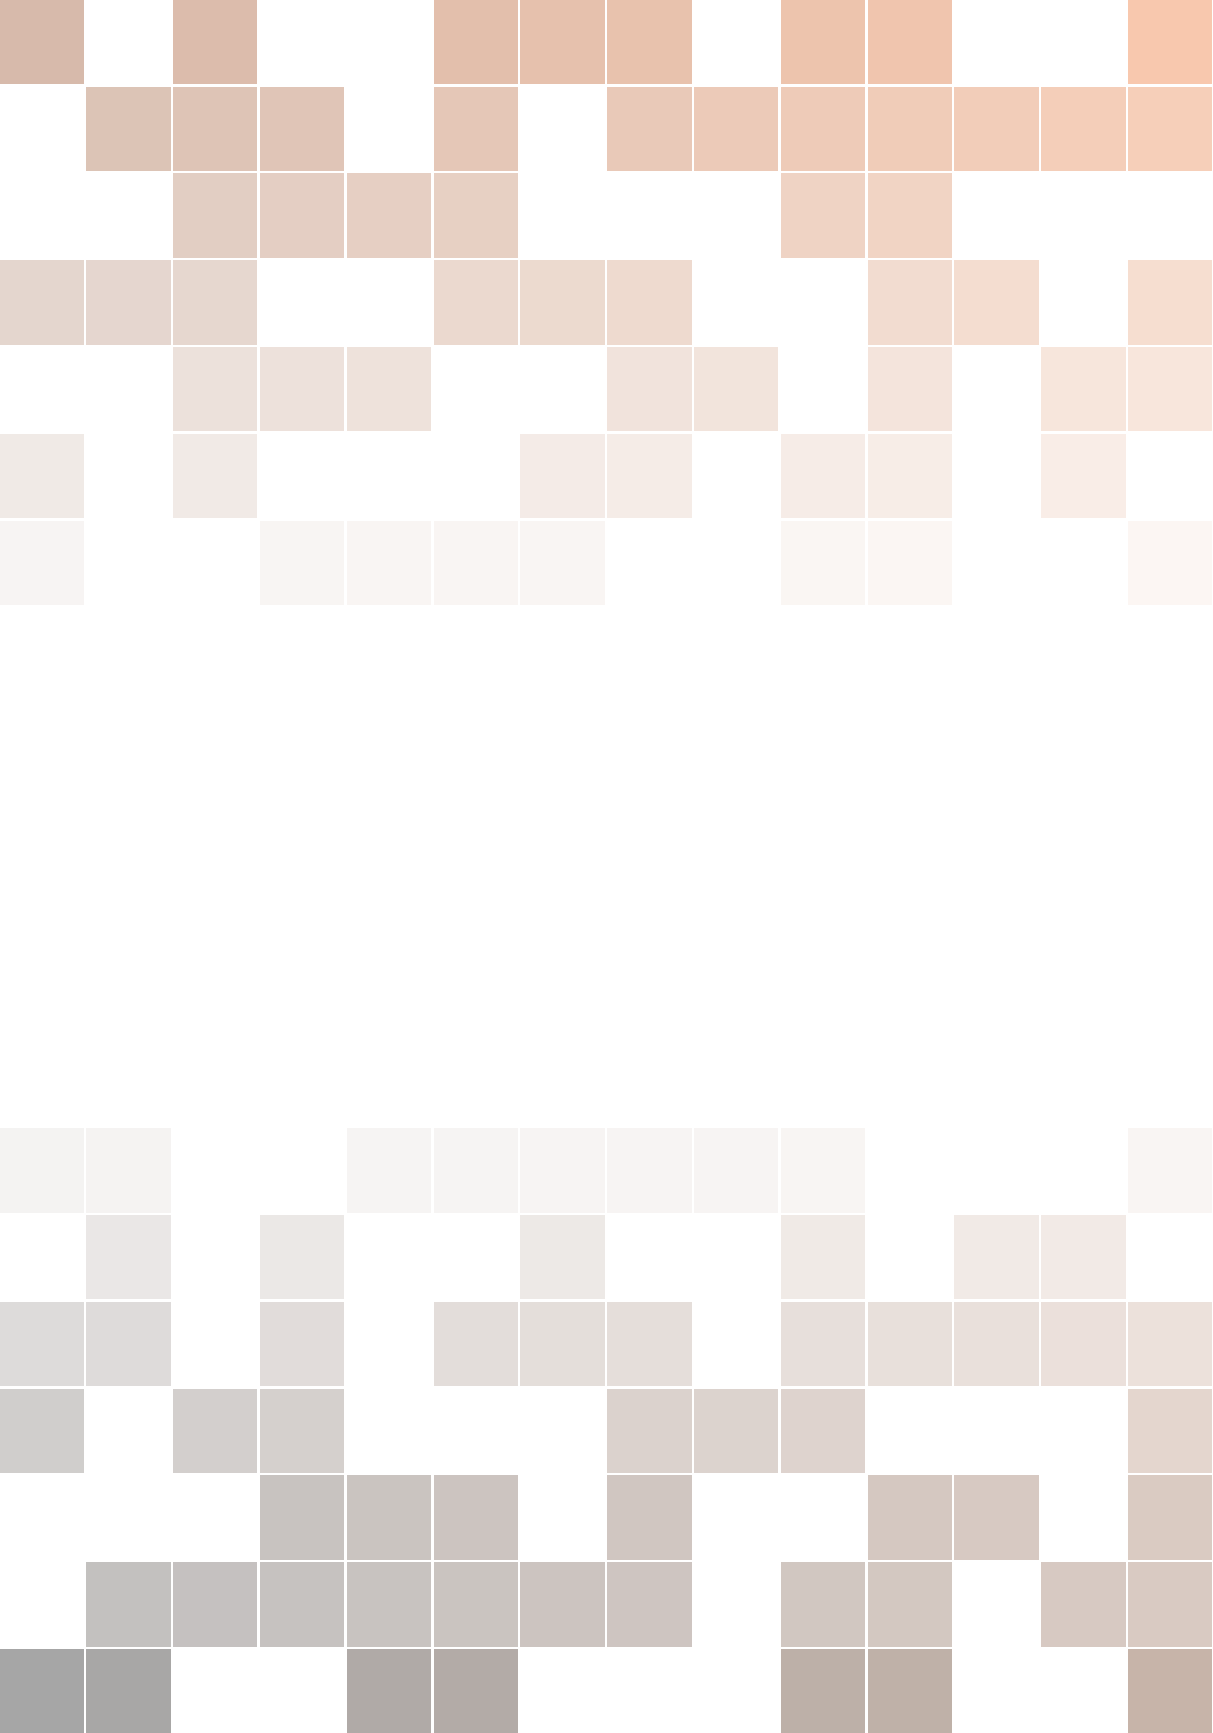
\includegraphics[width=\paperwidth]{background.pdf}};
\draw (current page.center) node [fill=ocre!30!white,fill opacity=0.6,text opacity=1,inner sep=1cm]{\Huge\centering\bfseries\sffamily\parbox[c][][t]{\paperwidth}{\centering Exerzitien zur Dreifaltigkeit\\[15pt] % Book title
{\Large inspiriert von «Der Göttliche Tanz»}\\[20pt] % Subtitle
{\huge Dona Mommsen}}}; % Author name
\end{tikzpicture}
\vfill
\endgroup

%----------------------------------------------------------------------------------------
%	COPYRIGHT PAGE
%----------------------------------------------------------------------------------------

\newpage
~\vfill
\thispagestyle{empty}

\noindent Copyright \copyright\ 2019 Dona Mommsen\\ % Copyright notice

%\noindent \textsc{Published by Publisher}\\ % Publisher

%\noindent \textsc{book-website.com}\\ % URL

%\noindent Licensed under the Creative Commons Attribution-NonCommercial 3.0 Unported License (the ``License''). You may not use this file except in compliance with the License. You may obtain a copy of the License at \url{http://creativecommons.org/licenses/by-nc/3.0}. Unless required by applicable law or agreed to in writing, software distributed under the License is distributed on an \textsc{``as is'' basis, without warranties or conditions of any kind}, either express or implied. See the License for the specific language governing permissions and limitations under the License.\\ % License information, replace this with your own license (if any)

\noindent \textit{In Arbeit seit Januar 2019} % Printing/edition date

%----------------------------------------------------------------------------------------
%	TABLE OF CONTENTS
%----------------------------------------------------------------------------------------

\usechapterimagefalse % If you don't want to include a chapter image, use this to toggle images off - it can be enabled later with \usechapterimagetrue

\chapterimage{chapter_head_1.pdf} % Table of contents heading image

\pagestyle{empty} % Disable headers and footers for the following pages

\tableofcontents % Print the table of contents itself

\cleardoublepage % Forces the first chapter to start on an odd page so it's on the right side of the book

\pagestyle{fancy} % Enable headers and footers again

%----------------------------------------------------------------------------------------
%	PART
%----------------------------------------------------------------------------------------
\part{Meditationen}

%\chapterimage{chapter_head_2.pdf} % Chapter heading image

\chapter{3x4 Meditationen}
\newpage
\section{Der Glanz auf Moses Gesicht}
\index{Glanz!Mose}

\textbf{\textit{S(t,t) | Gott, Jahwe | Spiegelung}}
\index{Sozialisierung S(t,t)}
\index{Gott!Jahwe}
\index{Spiegelung}

\biblerefformat{kurz}
\bibleverse{Ex}(34:27-35)
\begin{BibelSt}
Dann sprach der Herr zu Mose: Schreib diese Worte auf! Denn aufgrund dieser Worte schließe ich mit dir und mit Israel einen Bund. Mose blieb dort beim Herrn vierzig Tage und vierzig Nächte. Er aß kein Brot und trank kein Wasser. Er schrieb die Worte des Bundes, die zehn Worte, auf Tafeln. Als Mose vom Sinai herunterstieg, hatte er die beiden Tafeln der Bundesurkunde in der Hand. Während Mose vom Berg herunterstieg, wusste er nicht, dass die Haut seines Gesichtes Licht ausstrahlte, weil er mit dem Herrn geredet hatte. Als Aaron und alle Israeliten Mose sahen, strahlte die Haut seines Gesichtes Licht aus und sie fürchteten sich, in seine Nähe zu kommen. Erst als Mose sie rief, kamen Aaron und alle Sippenhäupter der Gemeinde zu ihm zurück und Mose redete mit ihnen. Dann kamen alle Israeliten herbei und er übergab ihnen alle Gebote, die der Herr ihm auf dem Sinai mitgeteilt hatte.  Als Mose aufhörte, mit ihnen zu reden, legte er über sein Gesicht einen Schleier.  Wenn Mose zum Herrn hineinging, um mit ihm zu reden, nahm er den Schleier ab, bis er wieder herauskam. Wenn er herauskam, trug er den Israeliten alles vor, was ihm aufgetragen worden war.  Wenn die Israeliten das Gesicht des Mose sahen und merkten, dass die Haut seines Gesichtes Licht ausstrahlte, legte er den Schleier über sein Gesicht, bis er wieder hineinging, um mit dem Herrn zu reden.
\end{BibelSt}
\subsection{Impuls}
\begin{impuls}
\begin{description}
\item[Gespiegeltes Wissen.] "Gespiegeltes Wissen ist kein 'logisches Wissen', sondern reflektiertes und empfangenes Wissen. Deshalb ist es so schwierig, einem Menschen Gott … oder die Liebe zu beweisen, wenn er nicht selbst schon Empfänger geworden ist. Tatsächlich ist es fast unmöglich. Erinnern Sie sich, wie Moses Gesicht leuchtete, als er den Blick Gottes empfangen hatte und mit Wahrhaftigkeit und Liebe angesehen worden war? Und doch verschleierte er sein Gesicht, als er seinem Volk gegenübertrat. Das ist ein grosses Symbol. Alle Menschen müssen als sie selbst und für sie selbst angesehen werden und den Blick Gottes ganz persönlich empfangen. Es reicht nicht, sich auf das Sehen oder Gesehenwerden eines anderen zu verlassen."\footnote{\cite[48]{Tanz}}
\item[Auszeiten und Orte der Begegnung.] Mose ist unterwegs in eine ungewisse Zukunft. Er hat die Verantwortung für ein ganzes Volk. Der Berg Sinai ist sein Ort der Begegnung mit Gott. Dieser Ort ist Mose vorbehalten, niemand sonst darf den Berg besteigen. 
\footnote{
\biblerefformat{kurz}
\bibleverse{Ex}(19:12)
}
Moses nimmt sich Zeit, zieht sich für 40 Tage zurück. Dabei ist dies schon das zweite Mal, dass Moses Gott auf dem Sinai sucht und findet. während der ersten Begegnung führte die Abwesenheit von Moses dazu, dass die Israeliten das Goldene Kalb fertigten.
\footnote{
\biblerefformat{kurz}
\bibleverse{Ex}(32:)
}
Trotzdem nimmt sich Moses eine zweite "Auszeit" und zieht sich für längere Zeit zurück. Während der Zeit zählt nur die Begegnung mit Gott, selbst auf die Gefahr hin dass jene, die ihm anvertraut sind, in seiner Abwesenheit wieder vom Weg abkommen und anderen Götzen nachlaufen. 
\item[Tafeln — den Bund fassbar machen.] Die ersten Tafeln, welche Moses aus Enttäuschung über das Goldene Kalb zerstört hatte, waren von Gott selber geschrieben. 
\footnote{
\biblerefformat{kurz}
\bibleverse{Ex}(31:18),
\biblerefformat{kurz}
\bibleverse{Ex}(32:19)
}
Nun ist Moses wieder auf dem Sinai, und diesmal schreibt er die Worte des Bundes selber auf die Tafeln. Diese Tafeln sind eine Hilfe, um die Gegenwart des unsichtbaren Gottes fassbar, greifbar zu machen. Die Mesusa, die Schriftrolle am Türpfosten, soll Gottes Wort und seine Gegenwart auch im Alltag sichtbar und greifbar machen.

\item[Ein unmerklicher Prozess.] Moses konzentriert sich auf die Kommunikation. Er empfängt von Gott die Worte, die er auf die Tafeln schreibt, und er gibt diese Worte an die Israeliten weiter. In dem Zusammensein mit Gott passiert jedoch eine Veränderung, dessen er sich selber nicht bewusst ist. Er erfährt eine "Erleuchtung", ein Glanz, der von ihm ausstrahlt. Als er dem Volk die Tafeln und die Worte Gottes überbringt, wirken nicht nur seine Worte, sondern auch seine Ausstrahlung, auch wenn er sie zu verschleiern versucht.
\end{description}

\begin{itemize}
\texitit{
    \item Ich darf mir längere Auszeiten nehmen. 
    \item Gibt es einen Ort an dem ich mich Gott nahe fühle? Wo ist mein Ort, wo ich mich zurückziehen und wohin ich immer wieder zurückkehren möchte?
    \item Wo ist mein Ort der Begegnung mit Gott im Alltag?
    }
\end{itemize}

\end{impuls}
\subsection{du spiegelst mein gesicht}
\cite{KHH} vom 8.9.
\begin{gedicht}
\begin{verse}
weiher meiner kindheit\\
versteckt im wald\\
umstanden von riedgrass\\
über das goldene käfer laufen\\
du spiegelst mein gesicht\\
und nebelstreifen\\
schleifen darüber\\!
mir wird schwindlig vor freude\\
weil du da bist\\
su-su-sirren die libellen\\
kräuselt das wasser\\
und du bist noch da\\
und er ist noch da\\
der ewige-eine\\
dessen gesicht mich\\
aus der tiefe anschaut
\end{verse}
\end{gedicht}
\subsection{Lied: Qui regarde vers Dieu (65/66)}
\begin{lied}
Qui regarde vers Dieu resplendira sur son visage,\\plus d’amertume sur son visage, plus d'amertume sur son visage.
\biblerefformat{kurz}
\bibleverse{Ps}(34:6)
\end{lied}

\subsection{Gebet}
Wer geduldig ist und in einen unerlässlichen Reifungsprozess einwilligt, erlebt den Tag, an dem sich sein inneres Wesen auferbaut hat – ohne dass er darum wusste.\footnote{\cite{FR-heute} vom 12.1.}
\newpage
\section{Die Verklärung Jesu}
\index{Glanz!Jesu}

\textbf{\textit{E(t,e) | Jesus | Spiegelung}}
\index{Externalisierung E(t,e)}
\index{Jesus!Verklärung}
\index{Spiegelung}

\biblerefformat{kurz}
\bibleverse{Mt}(17:1-9)
\begin{BibelSt}
Sechs Tage danach nahm Jesus Petrus, Jakobus und dessen Bruder Johannes beiseite und führte sie auf einen hohen Berg.  Und er wurde vor ihren Augen verwandelt; sein Gesicht leuchtete wie die Sonne und seine Kleider wurden blendend weiß wie das Licht.  Da erschienen plötzlich vor ihren Augen Mose und Elija und redeten mit Jesus.  Und Petrus sagte zu ihm: Herr, es ist gut, dass wir hier sind. Wenn du willst, werde ich hier drei Hütten bauen, eine für dich, eine für Mose und eine für Elija.  Noch während er redete, warf eine leuchtende Wolke ihren Schatten auf sie und aus der Wolke rief eine Stimme: Das ist mein geliebter Sohn, an dem ich Gefallen gefunden habe; auf ihn sollt ihr hören.  Als die Jünger das hörten, bekamen sie große Angst und warfen sich mit dem Gesicht zu Boden.  Da trat Jesus zu ihnen, fasste sie an und sagte: Steht auf, habt keine Angst!  Und als sie aufblickten, sahen sie nur noch Jesus.  Während sie den Berg hinabstiegen, gebot ihnen Jesus: Erzählt niemand von dem, was ihr gesehen habt, bis der Menschensohn von den Toten auferstanden ist.
\end{BibelSt}

\subsection{Impuls}
\begin{impuls}
\begin{figure}
    \centering
    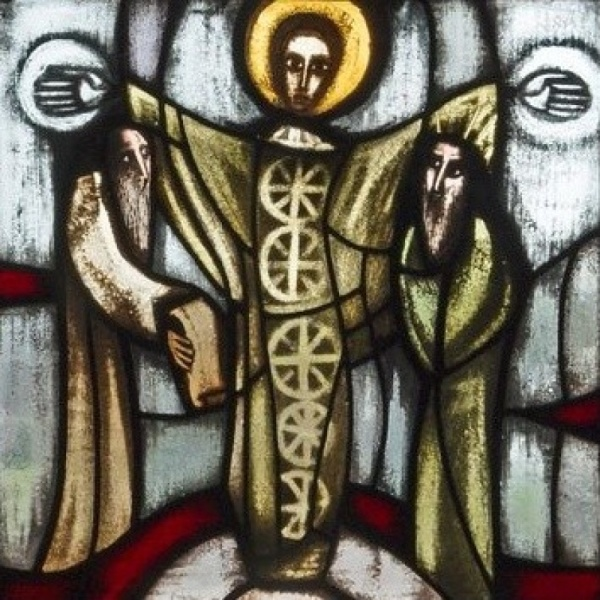
\includegraphics[scale=0.5]
{Pictures/ob_468a26_transfiguration-taize-2.jpg}
    \caption{Transfiguration, Kirche in Taizé}
    \label{fig:Bildmeditation}
\end{figure}

\begin{description}
\item[Petrus, Jakobus und Johannes]Es sind die ersten Jünger, 
\footnote{
\biblerefformat{kurz}
\bibleverse{Lk}(5:1-11); bei 
\biblerefformat{kurz}
\bibleverse{Mk}(4:14-20)
und
\biblerefformat{kurz}
\bibleverse{Mt}(4:18-20) ist auch noch Petrus Bruder Andreas dabei.
}
die Jesus von Anfang an begleitet haben, die auf dem Berg die Verklärung erleben. Bei \biblerefformat{kurz}
\bibleverse{Mt}(26:37) sind es ebenfalls diese drei Jünger, die er später bei seinem Gebet sind Gethsemani noch ein Stück weiter mit sich auf seinem Weg nimmt. Sie erhalten einen Augenblick die Herrlichkeit gezeigt, um sich daran zu erinnern, wenn sie Jesus auf dem Weg durch das Leiden und den Tod bis zur Auferstehung begleitet haben. 
\item[Die Stimme Gottes]«Dass ist mein geliebter Sohn, an dem ich meine Freude habe. Ihm sollt ihr gehorchen.» Die Jünger hören die Stimme Gottes, Jahwes, die ihnen Angst macht. Jesus ist der Freund an ihrer Seite, den sie begleiten - der sie begleitet.
\item[Berührung]Durch die Berührung von Jesus als Mensch werden die Jünger aufgerichtet, und es wird ihnen die Angst genommen. Gleichzeitig ist die Erscheinung der Verklärung vorbei. Es ist nur noch Jesus da.
\item[Mose und Elia] Jesus ist Teil der ewigen Dreifaltigkeit. Das bedeutet, das Mose und Elia Jesus bereits begegnet sind: im brennenden Dornbusch und im säuselnden Wind auf dem Horeb. 
\footnote{
\biblerefformat{kurz}
\bibleverse{Ex}(3:1-17),
\biblerefformat{kurz}
\bibleverse{1.Kön}(19:11-13)
}
Damals waren Mose und Elia Menschen auf dem Weg, die ihre Verantwortung in der Leitung des Volkes Gottes hatten. Nun ist der Dialog gespiegelt: Jesus ist in menschlicher Gestalt und hat die Erfüllung seines Auftrages noch vor sich, und Mose und Elia erscheinen ihm aus dem Jenseits. Nur in \biblerefformat{kurz}
\bibleverse{Lk}(9:31) wird erwähnt, worüber Mose und Elia mit Jesus sprechen: Jesus soll durch seinen Tod in Jerusalem Gottes Plan erfüllen. Die Erscheinung von Mose (als Vertreter des Gesetz) und Elia (als Prophet) soll dem Menschen Jesus zeigen, dass die Erfüllung Gottes Plans zur Herrlichkeit führt, auch wenn unsere menschlichen Vorstellungen übersteigt.
\item[Ausblick auf die Auferstehung]In der Verklärung wird die Grenze zwischen Tod und Leben fliessend. Mose und Elia erscheinen. Später wird den Jüngern Jesus als auferstandener Christus erscheinen. Hier auf dem Berg erleben die Jünger zum ersten Mal, dass des möglich ist, jemandem aus dem Jenseits zu begegnen. Als sie vom Berg heruntersteigen, gibt Jesus die Anweisung «Erzählt niemand von dem, was ihr gesehen habt, bis der Menschensohn von den Toten auferstanden ist.» Haben die Jünger wirklich verstanden, was Jesus damit gemeint hat?
\item[Hütten]Der Wunsch von Petrus, drei Hütten zu bauen, ist verständlich, aber der Glanz des Jenseits lässt sich nicht auf der Erde festhalten. Sie gehen auf dem Weg nach Jerusalem weiter und werden das Leiden von Jesus miterleben müssen. Gott, Jesus möchte ihnen in ihrem Herzen einen Vorrat an Hoffnung mitgeben, damit sie nicht beim Schrecken des Kreuzes stehenbleiben.

\end{description}

\end{impuls}

\subsection{weiss nicht was}
\cite{KHH} vom 30.8.
\begin{gedicht}
\begin{verse}
wende dich nicht weg\\
lichtwolke\\
überm wald\\
zieh den dunklen\\
mantel\\
nicht über\\
du verbirgst gewaltiges\\
aber ich weiss nicht\\
was\\!
wie kühl es ist\\
ist der sommer\\
vorüber?
\end{verse}
\end{gedicht}
\subsection{Lied: Oculi nostri (11)}
Oculi nostri ad Dominum Jesum, oculi notri ad Dominum nostrum.
\biblerefformat{kurz}
\bibleverse{Ps}(123:2)

\subsection{Gebet}
Sich nicht vor dem Leiden fürchten. In der Tiefe des Abgrunds kann es geschehen, dass die Freude sich in der Gemeinschaft mit Jesus Christus vollendet.\footnote{\cite{FR-heute} vom 5.2.}


\section{Trostworte an die Jünger}
\index{Geist!Erinnerung}

\textbf{\textit{C(e,e) | Geist | Erinnerung}}
\index{Kommunikation C(e,e)}

\biblerefformat{kurz}
\bibleverse{Joh}(14:15-26)
\begin{BibelSt}
Wenn ihr mich liebt, werdet ihr meine Gebote halten. Und ich werde den Vater bitten und er wird euch einen anderen Beistand geben, der für immer bei euch bleiben soll, den Geist der Wahrheit, den die Welt nicht empfangen kann, weil sie ihn nicht sieht und nicht kennt. Ihr aber kennt ihn, weil er bei euch bleibt und in euch sein wird. Ich werde euch nicht als Waisen zurücklassen, ich komme zu euch. Nur noch kurze Zeit und die Welt sieht mich nicht mehr; ihr aber seht mich, weil ich lebe und auch ihr leben werdet. An jenem Tag werdet ihr erkennen: Ich bin in meinem Vater, ihr seid in mir und ich bin in euch. Wer meine Gebote hat und sie hält, der ist es, der mich liebt; wer mich aber liebt, wird von meinem Vater geliebt werden und auch ich werde ihn lieben und mich ihm offenbaren. Judas - nicht der Iskariot - fragte ihn: Herr, wie kommt es, dass du dich nur uns offenbaren willst und nicht der Welt? Jesus antwortete ihm: Wenn jemand mich liebt, wird er mein Wort halten; mein Vater wird ihn lieben und wir werden zu ihm kommen und bei ihm Wohnung nehmen. Wer mich nicht liebt, hält meine Worte nicht. Und das Wort, das ihr hört, stammt nicht von mir, sondern vom Vater, der mich gesandt hat.
Das habe ich zu euch gesagt, während ich noch bei euch bin. Der Beistand aber, der Heilige Geist, den der Vater in meinem Namen senden wird, der wird euch alles lehren und euch an alles erinnern, was ich euch gesagt habe.
\end{BibelSt}

\subsection{Impuls}
\begin{impuls}
\begin{description}
\item[Erinnerung]«Wir haben versucht, Gott durch objektiviertes Wissen kennenzulernen, und das Ergebnis ist eine langweilige Schwarzweiss-Kopie, weil wir nicht selbst beteiligt sind. … Tatsache ist aber: Menschen begeistern sich nur für etwas, was sie in irgendeiner Weise einschliesst. Das weiss Gott, und deshalb schliesst er uns in sein eigenes Wissen ein – in dem er den Heiligen Geist in uns hineingibt, den inneren Wissenden, der uns an alles erinnert. Erinnern kann man sich nur an etwas, was man schon einmal im Inneren wusste. Eine ganz andere Form von Begreifen, Verinnerlichen, wird uns hier gegeben.»\footnote{\cite{Tanz}, Seite 49f. mit Verweis auf 
\biblerefformat{kurz}
\bibleverse{Joh}(14:26)}
\item[Dreiklang-Einklang] «Ich bin in meinem Vater, ihr seid in mir und ich bin in euch» und der Geist der Wahrheit ist auch in den Jüngern, in mir, in allen, die durch das Gebot der Liebe vereint sind. Ich lausche den Schwingungen der Klangschale, die mich an diesen Einklang erinnert.
\item[den Auferstandenen sehen] Jesus erklärt den Jüngern, dass sie ihn sehen werden, selbst wenn er für die Welt nicht mehr sichtbar ist. Können Petrus, Jakobus und Johannes, die Zeugen der Verklärung, welche auch Moses und Elia sehen konnten, diese Worte besser verstehen? Die Erscheinung von Moses und Elia war eine erste Begegnung mit Menschen, die eigentlich schon lange tot sind («Externalisierung»). Der nächste Schritt in der Lernspirale besteht darin, diese Erfahrung mit den anderen Elementen zu kombinieren: Die Worte Jesu, das Gebot der Liebe, die ständige Gegenwart und die Einheit von Gott, Jesus und Geist. Auch wenn die Jünger den Zusammenhang noch nicht erfassen können, so kündigt ihnen Jesus an, dass die Kraft des Geistes später ermöglichen wird, diese Wahrheiten zu verinnerlichen.
\item[Liebe] Die Liebe ist der Schlüssel zur Einheit mit dem dreieinigen Gott. Wer liebt, erfüllt das Gebot, das zur Einheit mit Gott führt. Doch kann man liebe «gebieten»? Kann man Liebe definieren, beschreiben? Es ist der Geist in mir, der mich berührt, mich zu Tränen rührt und daran erinnert, was Liebe im Herzen bedeutet.
\end{description}
\end{impuls}

\subsection{Heiliger Geist - wer bist du?}
\cite{KHH} vom 22.5.
\begin{gedicht}
\begin{verse}
du\\
Heiliger Geist\\
wer bist du?\\
wind, flamme, gesang?\\
bist du das licht, das\\
alles in sich zusammenhält?\\
die wirklichkeit Gottes?\\
seine zärtlichkeit?\\
bist du die tiefe\\
innerlichkeit eines\\
menschen, der lächelt\\
weil er sich von\\
Gott angesehen weiss?
\end{verse}
\end{gedicht}
\subsection{Lied: Esprit consolateur (126)}
Esprit consolateur, amour de tout amour.

\subsection{Gebet}
Wissen, wo unser Herz ausruhen kann, heisst eine Wirklichkeit erfassen, die unseren Augen verborgen ist: Christus begleitet uns. Unser bedrücktes Herz lebt von neuem auf. Es beginnt, mitunter lautlos, zu singen: Der Atem deiner Liebe hat mich durchströmt, ich trete nicht auf der Stelle, ich gehe mit dir.\footnote{\cite{FR-heute} vom 7.2.}



\newpage
\section{Die Vision der Auferweckung Israels}
\index{Geist!Leben}
\index{Auferstehung!Auferweckung}

\textbf{\textit{I(e,t) | Jahwe | Geist}}
\index{Internalisierung I(e,t)}

\biblerefformat{kurz}
\bibleverse{Ezechiel}(37:1-14)
\begin{BibelSt}
Die Hand des HERRN legte sich auf mich und er brachte mich im Geist des HERRN hinaus und versetzte mich mitten in die Ebene. Sie war voll von Gebeinen. Er führte mich ringsum an ihnen vorüber und siehe, es waren sehr viele über die Ebene hin; und siehe, sie waren ganz ausgetrocknet. Er fragte mich: Menschensohn, können diese Gebeine wieder lebendig werden? Ich antwortete: GOTT und Herr, du weißt es. Da sagte er zu mir: Sprich als Prophet über diese Gebeine und sag zu ihnen: Ihr ausgetrockneten Gebeine, hört das Wort des HERRN! So spricht GOTT, der Herr, zu diesen Gebeinen: Siehe, ich selbst bringe Geist in euch, dann werdet ihr lebendig. Ich gebe euch Sehnen, umgebe euch mit Fleisch und überziehe euch mit Haut; ich gebe Geist in euch, sodass ihr lebendig werdet. Dann werdet ihr erkennen, dass ich der HERR bin. Da sprach ich als Prophet, wie mir befohlen war; und noch während ich prophetisch redete, war da ein Geräusch: Und siehe, ein Beben: Die Gebeine rückten zusammen, Bein an Bein. Und als ich hinsah, siehe, da waren Sehnen auf ihnen, Fleisch umgab sie und Haut überzog sie von oben. Aber es war kein Geist in ihnen. Da sagte er zu mir: Rede als Prophet zum Geist, rede prophetisch, Menschensohn, sag zum Geist: So spricht GOTT, der Herr: Geist, komm herbei von den vier Winden! Hauch diese Erschlagenen an, damit sie lebendig werden! Da sprach ich als Prophet, wie er mir befohlen hatte, und es kam der Geist in sie. Sie wurden lebendig und sie stellten sich auf ihre Füße - ein großes, gewaltiges Heer.
Er sagte zu mir: Menschensohn, diese Gebeine sind das ganze Haus Israel. Siehe, sie sagen: Ausgetrocknet sind unsere Gebeine, unsere Hoffnung ist untergegangen, wir sind abgeschnitten. Deshalb tritt als Prophet auf und sag zu ihnen: So spricht GOTT, der Herr: Siehe, ich öffne eure Gräber und hole euch, mein Volk, aus euren Gräbern herauf. Ich bringe euch zum Ackerboden Israels. Und ihr werdet erkennen, dass ich der HERR bin, wenn ich eure Gräber öffne und euch, mein Volk, aus euren Gräbern heraufhole. Ich gebe meinen Geist in euch, dann werdet ihr lebendig und ich versetze euch wieder auf euren Ackerboden. Dann werdet ihr erkennen, dass ich der HERR bin. Ich habe gesprochen und ich führe es aus - Spruch des HERRN.
\end{BibelSt}

\subsection{Impuls}
\begin{impuls}
\begin{description}
\item[Wirken des Geistes] «Der Heilige Geist … lässt uns wachsen und hält uns verletzlich. Fur das Leben und die Liebe. Bezeichnend dabei ist, dass die wichtigsten biblischen Metaphern für den Heiligen Geist immer dynamisch, energisch, und beweglich sind.»\footnote{\cite{Tanz} S. 54}
\item[Prophet] Diese Bibelstelle zeigt die Verinnerlichung (Internalisierung) auf unterschiedlichen Ebenen. Als Teil der Vision sieht der Prophet wie die Kraft Gottes den ausgetrockneten Gebeinen wieder Leben schenkt. In der Vision ist die Schaffung des Körpers aus Fleisch getrennt von der Kraft des Geistes, der den Menschen wieder Leben einhaucht. Die Verinnerlichung ist aber noch viel umfassender. Gott zeigt dem Propheten nicht nur seine Kraft, sondern auch, dass diese durch das Wort des Propheten zur Entfaltung kommt. Ezechiel überlässt Gott die Entscheidung, wo und wie er seine Macht zeigen möchte. Gott fragt: «Ist es möglich?» und Ezechiel antwortet voll Vertrauen «GOTT und Herr, du weisst es.» Gott beschränkt sich nicht darauf, das seine Kraft und das Wirken des Geistes zu demonstrieren. Er fordert den Propheten bewusst auf: Sprich Du zu den Gebeinen; rufe Du den Geist aus den vier Winden herbei. In der Vision lässt Gott den Propheten seine Aufgabe als Vermittler erfahren und erlernen.
\item[Ackerboden] Aus der Perspektive der Menschen, die alle Hoffnung verloren haben (die ausgetrockneten Gebeine), sind es die Worte des Propheten, die Gottes Wirken ankündigen und real werden lassen. Als Teil dieses neuen Lebens werden sie auf ihren Ackerboden zurückgebracht. Sie werden wieder Teil des Kreislaufs des Lebens und der Natur.
\end{description}
\end{impuls}

\subsection{ich hüte das wort}
\cite{KHH} vom 4.6
\begin{gedicht}
\begin{verse}
frau unter den sternen\\
wer bist du?\\!
ich hüte das wort\\
unterm kelch\\
und achte auf\\
das brausen\\
des geistes\\
in den lüften
\end{verse}
\end{gedicht}

\subsection{Der Prophet — der Abschied}
«Ich drücke nur in Worten für euch aus, was ihr in Gedanken selber wisst. Und was ist Wissen in Worten anderes als ein Schatten wortlosen Wissens? Eure Gedanken und meine Worte sind Wellen aus einem versiegelten Gedächtnis, das Bericht gibt von unseren gestrigen Tagen, und von den alten Tagen, da die Erde weder uns noch sich selber kannte, und von den Nächten, da die Erde in Verwirrung aufgewühlt war. Weise sind zu euch gekommen, um euch von ihrer Weisheit zu geben. Ich kam, um von eurer Weisheit zu nehmen: Und, seht, ich habe gefunden, was größer ist als Weisheit. Es ist ein Flammengeist in euch, der sich immer mehr steigert, während ihr, seiner Entfaltung ungeachtet, das Vergehen eurer Tage beklagt. Es ist das Leben auf der Suche nach Leben in Körpern, die vor dem Grab erzittern.
Hier gibt es keine Gräber. Diese Berge und Ebenen sind eine Wiege und ein Trittstein. Wann immer ihr an dem Feld vorbeikommt, in dem ihr eure Vorfahren beigesetzt habt, schaut richtig hin, und ihr werdet euch und eure Kinder Hand in Hand tanzen sehen.»\footnote{\cite{prophet}S. 116}

\subsection{Lied: I am sure I shall see (127)}
I am sure I shall see the goodness of the Lord in the land of the living. Yes, I shall see the goodness of our God, hold firm, trust in the Lord. \biblerefformat{kurz}
\bibleverse{Ps}(27:13)

\subsection{Gebet}
Scheinbar entbehrt die endlose Wiederholung der gleichen Worte im Gebet jeder Spontaneität. Aber nach langem Warten brechen unversehens innere Quellen auf, eine Fülle, die Gegenwart des Heiligen Geistes, die immer wieder aufrüttelt.
\footnote{\cite{FR-heute} vom 16.5.}

\newpage
\section{Die Heilung einer blutflüssigen Frau}
\index{Heilung}

\textbf{\textit{S(t,t) | Jesus | Berührbarkeit}}
\index{Sozialisierung S(t,t)}
\index{Jesus}
\index{Berührbarkeit}


\biblerefformat{kurz}
\bibleverse{Mt}(9:20-22)
\begin{BibelSt}
Und siehe, eine Frau, die schon zwölf Jahre an Blutfluss litt, trat von hinten heran und berührte den Saum seines Gewandes; denn sie sagte sich: Wenn ich auch nur sein Gewand berühre, werde ich geheilt. Jesus wandte sich um, und als er sie sah, sagte er: Hab keine Angst, meine Tochter, dein Glaube hat dich gerettet! Und von dieser Stunde an war die Frau geheilt. 
\end{BibelSt}

\subsection{Impuls}
\begin{impuls}
\begin{description}
\item[Isolierte Frau] Die Periode ist ein Teil des Kreislaufes der Natur, der den weiblichen Körper ständig verändert, so wie die Jahreszeiten. Die Natur der Frau ist Teil des Kreislaufes des Lebens, der Schöpfung; doch nach dem Gesetz macht dieser Blutfluss unrein. Wer eine Frau während ihrer Periode berührt, wird dadurch selber unrein \biblerefformat{kurz}\bibleverse{Lev}(15:19). Durch dieses Gesetz ist die Frau nun schon seit 12 Jahren isoliert. Jesus zu berühren ist aus der Sicht des Gesetzes ein grosses Vergehen, weil dadurch er dadurch selber unrein wird. Indem die Frau die Nähe zu Jesus sucht und aus ihrem Glauben heraus die Grenzen des Gesetzes überwindet, entsteht eine Beziehung, in der die Kraft Gottes wirkt. Gott möchte unser Heil und unsere Heilung.

\item[Berührbarkeit] «Sie haben sicher schon bemerkt, dass Jesus keine Checkliste abhakt, bevor er jemanden heilt. Er fragt nur: "Lässt du zu, dass ich dich berühre? Wenn ja, dann kann es losgehen." Die Berührbaren werden geheilt. So einfach ist das. … Es gibt nur eine Frage: \textit{Willst du geheilt werden?} Wenn die Antwort verletzlich, vertrauensvoll oder zuversichtlich ist, dann fliesst der Fluss und der Mensch wird geheilt.» \footnote{\cite{Tanz} S. 55}
In dieser Bibelstelle geschieht dieser Fluss der Kraft ganz ohne Worte. 
\footnote{Bei \biblerefformat{kurz}\bibleverse{Mk}(5:21-43) und \bibleverse{Lk}(8:43-48) erklärt die Frau erst den Umstehenden, warum sie es gewagt hat Jesus zu berühren, und erklärt, dass diese Berührung sie tatsächlich geheilt hat.}
Es genügt die Berührung, und als Jesus die Frau ansieht, weiss er um ihre Not und ihren Glauben.

\item[Ausbluten] Der gesunde Zyklus ist ein Wechsel von Ausfluss und Sammlung. Wenn dieser Zyklus gestört ist, und der Mensch nur noch ausblutet, leidet er/sie unter dem ständigen Verlust an Lebenskraft und Lebensfreude. Dies gilt auch im übertragenen Sinne. Wenn ich das Gefühl habe auszubluten, brauche ich die Berührung Gottes, um den Kreislauf des Verschenkens und der Sammlung wieder ins Gleichgewicht zu bringen.
\end{description}

%\begin{itemize}
%\texitit{
%\item 
   
%    }
%\end{itemize}

\end{impuls}
\subsection{Rühre mich an}

\begin{gedicht}
\begin{verse}
Ich möchte dich berühren, Herr\\
und wenn es nur der Saum deines Gewandes ist,\\
den ich halten kann\\!

Ich möchte dich berühren, Herr\\
und wenn es nur ein Wort deiner Botschaft ist,\\
die ich fassen kann.\\!

Ich möchte dich berühren, Herr,\\
möchte mich heran-tasten an dich.\\!

Ich möchte dich berühren, Herr,\\
deinen Saum,\\
deinen Finger,\\
dein Wort.\\!

Ich möchte dich berühren, Herr,\\
und ahnen dein Gewand,\\
deine Hand,\\
deine Botschaft.\\!

Ich möchte dich berühren, Herr,\\
und fühlen die Kraft, die ausströmt,\\
die Wärme, die belebt,\\
das Leben, das heilt.\\!

Ich möchte dich berühren, Herr,\\
und ich wage es,\\!

Ich rühre dich an\\
Rühre du mich an, Herr,\\
fasse mich,\\
ergreife mich,\\
halte mich –\\
heile mich.\\
\poemauthorcenter{Marie-Lousie Langwald\footnote{\cite{biblFrauen} S. 40}}

\end{verse}
\end{gedicht}
\subsection{Lied: Voici Dieu qui vient à mon secours (142)}
\begin{lied}
Voici Dieu qui vient à mon secours, le Seigneur avec ceux qui me soutiennent. Je te chante, toi qui me relèves. Je te chante, toi qui me relèves. \biblerefformat{kurz}
\bibleverse{Ps}(54:6) und \bibleverse{Ps}(30:2)
\end{lied}

\subsection{Gebet}
Es wagen, sich über alles zu freuen, was Gott in uns und um uns vollbringt. Und alles, wofür man bei sich selbst und bei den anderen schwarz sieht, alles, was einem den Seelenfrieden raubt, löst sich auf.\footnote{\cite{FR-heute} vom 29.4}
\newpage
\section{Gott legt seinen Geist auf jung und alt}
\index{Glanz!Jesu}

\textbf{\textit{E(t,e) | Jahwe | Geist}}
\index{Externalisierung E(t,e)}
\index{Jahwe}
\index{Geist}

\biblerefformat{kurz}
\bibleverse{Num}(11:16-17.25-30)
\begin{BibelSt}
Da sprach der HERR zu Mose: Versammle mir siebzig von den Ältesten Israels, die du kennst, weil sie die Ältesten des Volkes und seine Listenführer sind; bring sie zum Offenbarungszelt! Dort sollen sie mit dir zusammen hintreten. Dann komme ich herab und rede dort mit dir. Ich nehme etwas von dem Geist, der auf dir ruht, und lege ihn auf sie. So können sie mit dir zusammen an der Last des Volkes tragen und du musst sie nicht mehr allein tragen. \!
Der HERR kam in der Wolke herab und redete mit Mose. Er nahm etwas von dem Geist, der auf ihm ruhte, und legte ihn auf die siebzig Ältesten. Sobald der Geist auf ihnen ruhte, redeten sie prophetisch. Danach aber nicht mehr.
Zwei Männer aber waren im Lager geblieben; der eine hieß Eldad, der andere Medad. Auch über sie kam der Geist. Sie gehörten zu den Aufgezeichneten, waren aber nicht zum Offenbarungszelt hinausgegangen. Auch sie redeten prophetisch im Lager. Ein junger Mann lief zu Mose und berichtete ihm: Eldad und Medad sind im Lager zu Propheten geworden. Da ergriff Josua, der Sohn Nuns, der von Jugend an der Diener des Mose gewesen war, das Wort und sagte: Mose, mein Herr, hindere sie daran! Doch Mose sagte zu ihm: Willst du dich für mich ereifern? Wenn nur das ganze Volk des HERRN zu Propheten würde, wenn nur der HERR seinen Geist auf sie alle legte! Dann zog sich Mose mit den Ältesten Israels in das Lager zurück.
\end{BibelSt}

\subsection{Impuls}
\begin{impuls}

\begin{description}
\item[]

\end{description}

\end{impuls}

\subsection{Heiliger Geist}
\cite{KHH} vom 5.6.
\begin{gedicht}
\begin{verse}
er kommt\\
   kommt\\
   kommt\\
durchkommt er\\
durch die zeit\\
hebt sie auf\\
wird gegenwart\\!

erwartet\\
uns\\
in der zukunft\\!
\end{verse}
\end{gedicht}
\subsection{Lied: Veni Creator, litanie (13)}
Veni Creator spiritus.

\subsection{Gebet}
\footnote{\cite{FR-heute} vom }

\newpage
\section{Die Samariterin am Brunnen}
\index{Jesus}

\textbf{\textit{C(e,e) | Jesus | Quelle}}
\index{Kommunikation C(e,e)}
\index{Quelle}

\biblerefformat{kurz}
\bibleverse{Joh}(4:5-26)
\begin{BibelSt}
So kam er zu einer Stadt in Samarien, die Sychar hieß und nahe bei dem Grundstück lag, das Jakob seinem Sohn Josef vermacht hatte. Dort befand sich der Jakobsbrunnen. Jesus war müde von der Reise und setzte sich daher an den Brunnen; es war um die sechste Stunde.
Da kam eine Frau aus Samarien, um Wasser zu schöpfen. Jesus sagte zu ihr: Gib mir zu trinken! Seine Jünger waren nämlich in die Stadt gegangen, um etwas zum Essen zu kaufen. Die Samariterin sagte zu ihm: Wie kannst du als Jude mich, eine Samariterin, um etwas zu trinken bitten? Die Juden verkehren nämlich nicht mit den Samaritern. Jesus antwortete ihr: Wenn du wüsstest, worin die Gabe Gottes besteht und wer es ist, der zu dir sagt: Gib mir zu trinken!, dann hättest du ihn gebeten und er hätte dir lebendiges Wasser gegeben. Sie sagte zu ihm: Herr, du hast kein Schöpfgefäß und der Brunnen ist tief; woher hast du also das lebendige Wasser? Bist du etwa größer als unser Vater Jakob, der uns den Brunnen gegeben und selbst daraus getrunken hat, wie seine Söhne und seine Herden? Jesus antwortete ihr: Wer von diesem Wasser trinkt, wird wieder Durst bekommen; wer aber von dem Wasser trinkt, das ich ihm geben werde, wird niemals mehr Durst haben; vielmehr wird das Wasser, das ich ihm gebe, in ihm zu einer Quelle werden, deren Wasser ins ewige Leben fließt. Da sagte die Frau zu ihm: Herr, gib mir dieses Wasser, damit ich keinen Durst mehr habe und nicht mehr hierherkommen muss, um Wasser zu schöpfen!
Er sagte zu ihr: Geh, ruf deinen Mann und komm wieder her! Die Frau antwortete: Ich habe keinen Mann. Jesus sagte zu ihr: Du hast richtig gesagt: Ich habe keinen Mann. Denn fünf Männer hast du gehabt und der, den du jetzt hast, ist nicht dein Mann. Damit hast du die Wahrheit gesagt. Die Frau sagte zu ihm: Herr, ich sehe, dass du ein Prophet bist. Unsere Väter haben auf diesem Berg Gott angebetet; ihr aber sagt, in Jerusalem sei die Stätte, wo man anbeten muss. Jesus sprach zu ihr: Glaube mir, Frau, die Stunde kommt, zu der ihr weder auf diesem Berg noch in Jerusalem den Vater anbeten werdet. Ihr betet an, was ihr nicht kennt, wir beten an, was wir kennen; denn das Heil kommt von den Juden. Aber die Stunde kommt und sie ist schon da, zu der die wahren Beter den Vater anbeten werden im Geist und in der Wahrheit; denn so will der Vater angebetet werden. Gott ist Geist und alle, die ihn anbeten, müssen im Geist und in der Wahrheit anbeten. Die Frau sagte zu ihm: Ich weiß, dass der Messias kommt, der Christus heißt. Wenn er kommt, wird er uns alles verkünden. Da sagte Jesus zu ihr: Ich bin es, der mit dir spricht.
\end{BibelSt}

\subsection{Impuls}
\begin{figure}
    \centering
    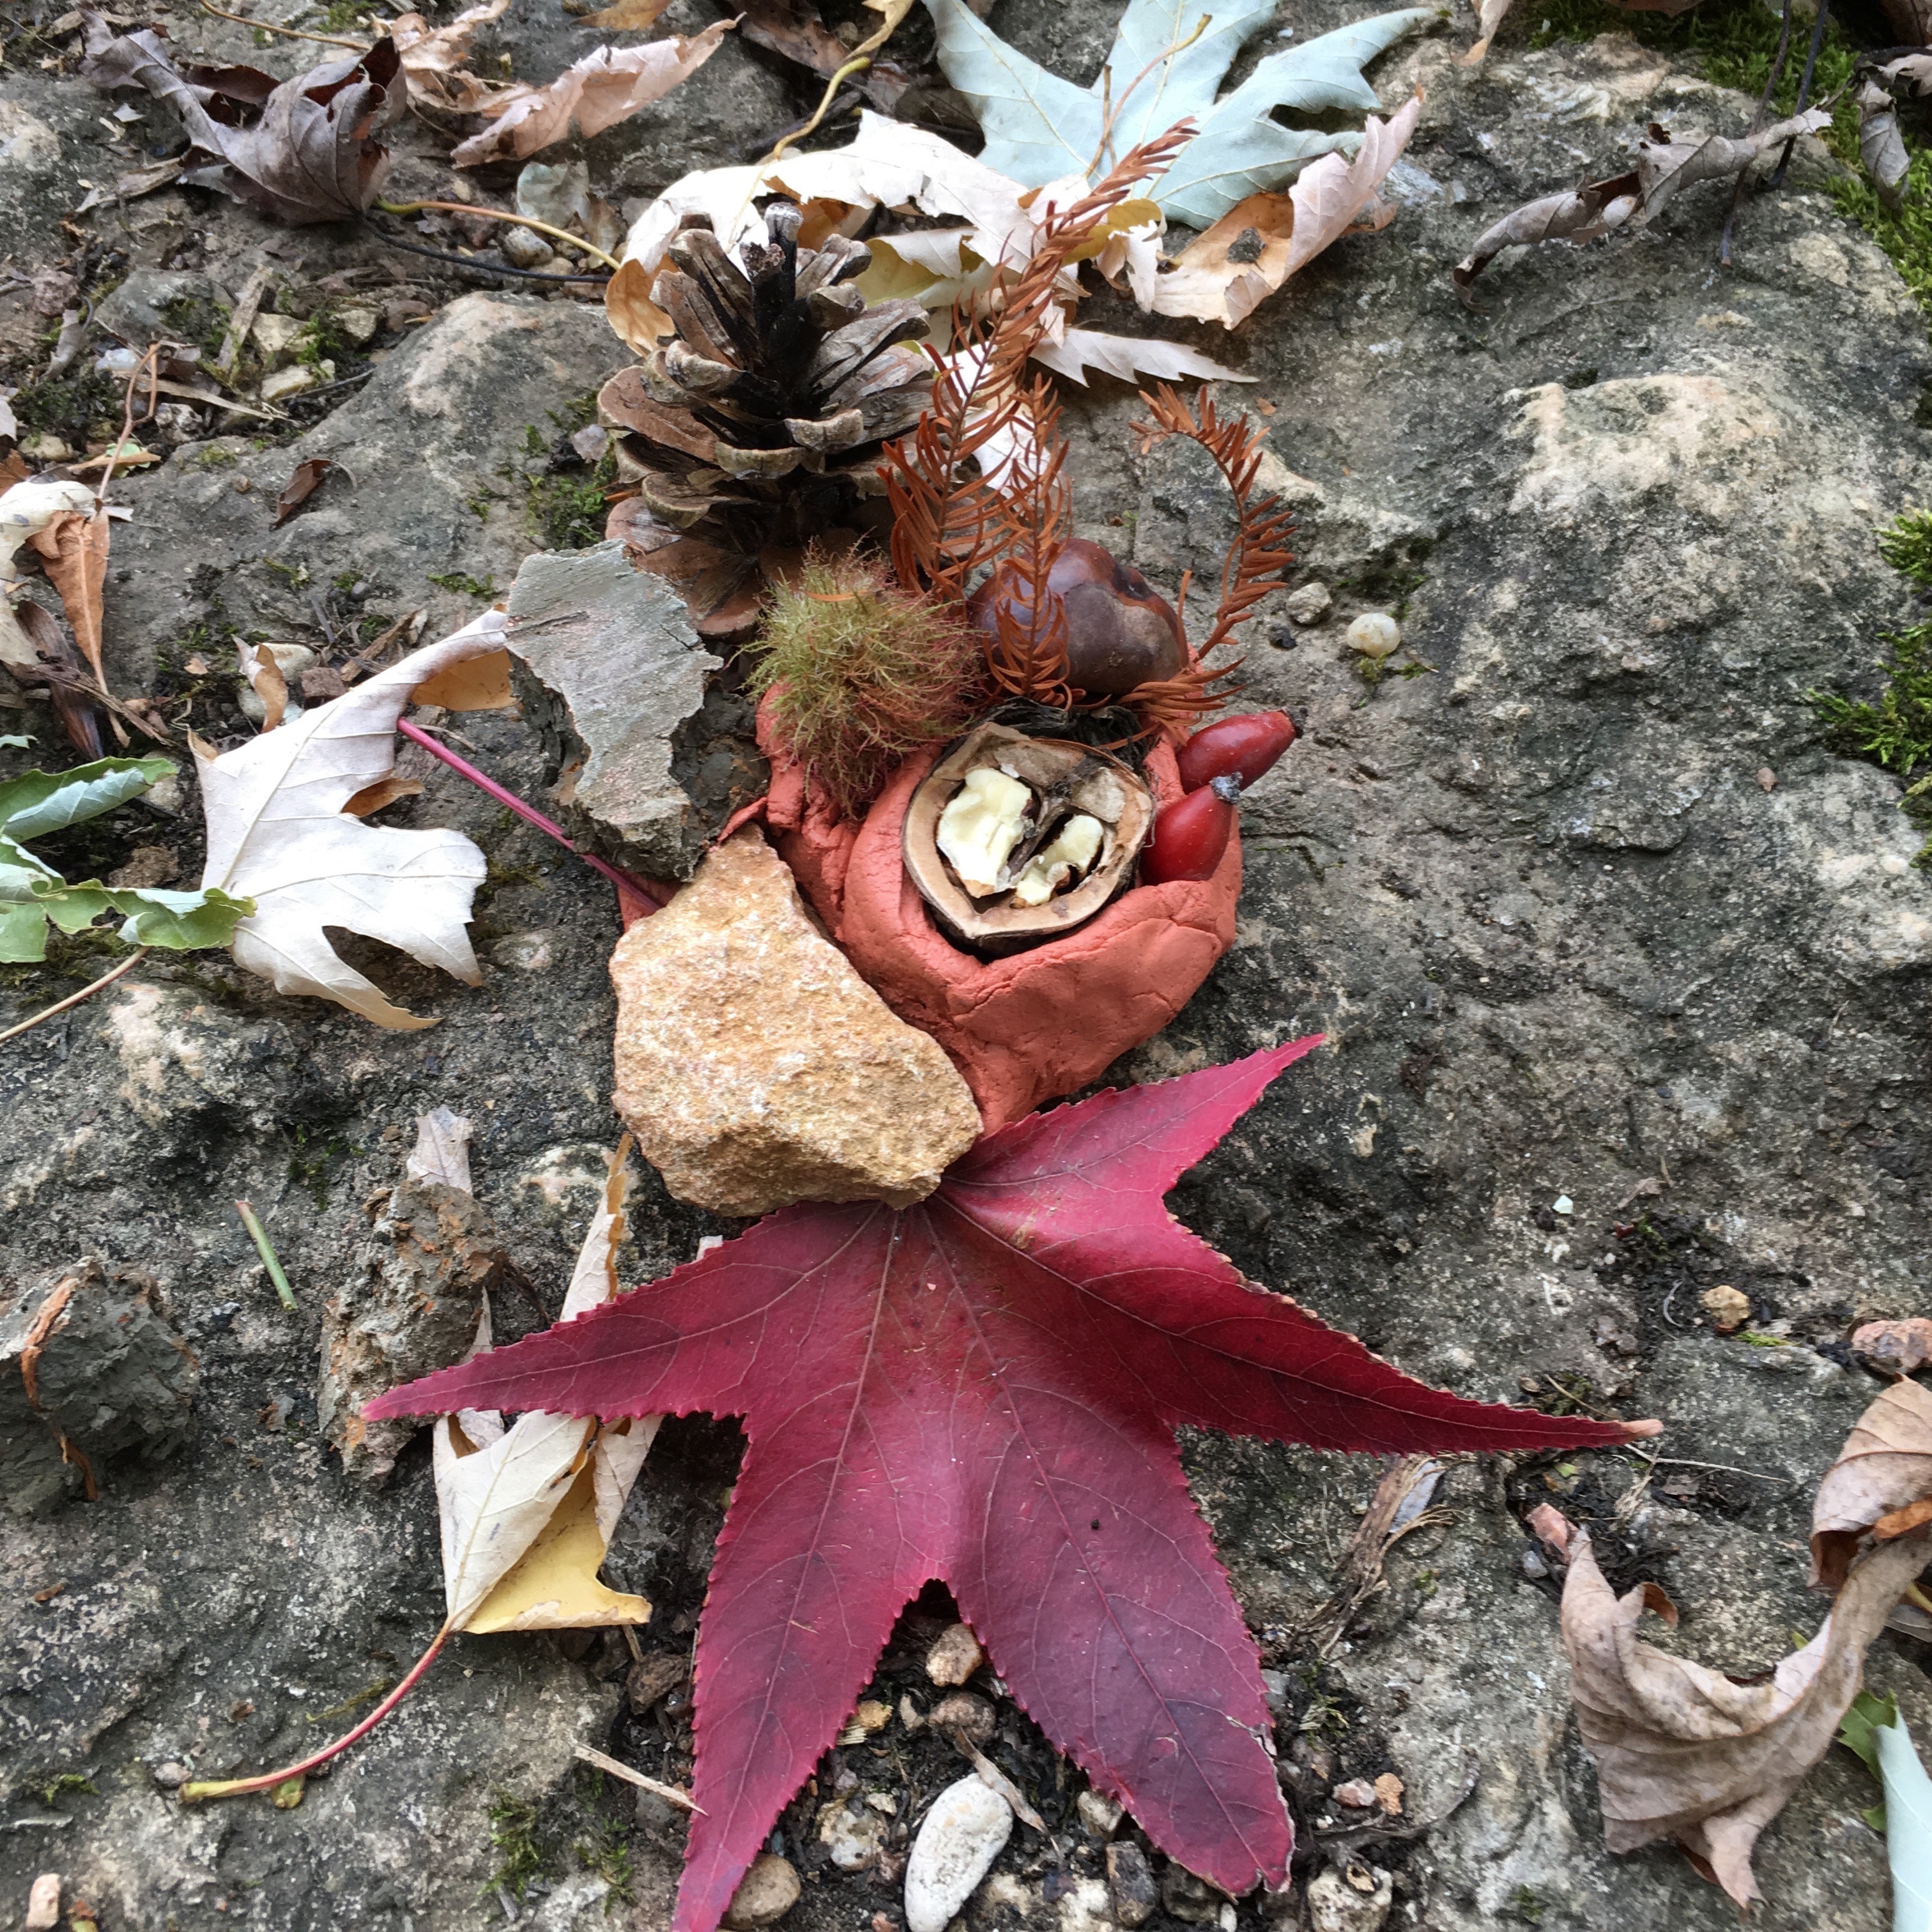
\includegraphics[scale=0.09]
{Pictures/2018-10-Gottesbild-Taize.jpg}
    \caption{Gottesbild, 25. Oktober 2018, Taizé}
    \label{fig:Bildmeditation}
\end{figure}
\begin{impuls}
\begin{description}
 \item[Gottesbilder: bei der Quelle]
 \begin{gedicht}
 \begin{verse}
 \\!
 Taizé — Pilgerweg des Vertrauens in einen Gott,  der für mich Geist — Energie, Wind — ist. Das Unfassbare ist mir am nächsten.\\!
 
Aus Erde geschaffen. Was lässt sich aus diesem Ton formen?\\!

Aufmerksam werden, für das, was mir am Wegrand geschenkt wird: Stein, Kastanie. 
Erinnerung an frühere Stationen auf dem Pilgerweg hier in Taizé. Den Ton formen um zu fassen, was mir am Wegrand geschenkt wird.\\
Nuss — ihr Kern enthält alles, um ein grosser, starker Baum zu werden. Tannzapfen, rote Blätter… Erinnerungen. Vergängliche Schönheit des Herbstes, selbst im Unkraut.\\!

Ich wollte zur Quelle kommen, doch der Teich ist ausgetrocknet. In der Ferne schwingt der Psalm mit: «Wie der Hirsch lechzt nach frischem Wasser»… Ausgetrockneter Teich, Lehmboden. Aus der Erde geschaffen … kein Meissen-Porzellan. Der Versuch, in dem instabilen Gefäss zu fassen, was mir geschenkt wird. \\!

Zerbrechlich. Vergänglich.\\!

Echo einer Bibelstelle: Was weiss der Ton über seinen Schöpfer? 
Sich kein Bild von Gott machen. Und nun forme ich nicht Gott, sondern meine zu ahnen, wie Gott mich formen möchte.\\!
 \end{verse}
 \end{gedicht}
 \item[Auf dem Weg und beim Gotteswortgärtchen] 
 \begin{gedicht}
 \begin{verse}
 \\!
 Vergänglich die Geschenke, zerbrechlich der Ton. Gehärtet im Wind und Feuer des Geistes, und doch zerbrechlich. Der Versuch, zusammenzuhalten. Wissen um die Vergänglichkeit, und doch das Zerbrechen verhindern — hinauszögern.\\!
 
Getragen in der Hand des Schöpfers. Getragen sein. Tragen. Weitergehen auf dem Pilgerweg des Vertrauens zu meinem Gotteswortgärtchen.\\!

Ikone der Begegnung mit der Samariterin am Brunnen. Das Echo des lebendigen Wassers nach der ausgetrockneten Quelle. Tränen. Erinnerungen.\\!

Mein Gottesbild auf dem Pilgerweg des Vertrauens, gewickelt in Zeitungspapier, in eine Kartonschachtel gelegt. Eine Krippe? Wird hier ein neues Gottesbild geboren?
\end{verse}
 \end{gedicht}
\end{description}
\end{impuls}

\subsection{die samariterin am brunnen}
\cite{KHH} vom 17.3
\begin{gedicht}
\begin{verse}
sie sagen, ich sei eine hure.\\
ein leichtes mädchen\\
ich mit meinen stöckelschuhen\\
den klingenden armbändern\\
dem roten kleid und dem weigenden gang\\
sie gehn mir aus dem weg\\
wenigstens tagsüber\\!

darum laufe ich\\
in der hitze zum brunnen\\
ich ertrage die blicke\\
der frauen nicht\\!

jetzt bist du da\\
fremder mann\\
du batest um einen schluck wasser\\
du, der fremde\\!

nicht die hure sahst du in mir\\
nicht die frau\\
nicht die fremde und andersgläubige\\
su sahst in mir den menschen\\
der hinter der schminke weint\\
und gabst mir aus deiner quelle\\
wasser des heils und der vergebung\\
auf dass ich lebe\\
und alle herbeirufe\\
zu deinem brunnen
\end{verse}
\end{gedicht}

\subsection{Lied: De noche (12)}
De noche iremos, de noche que para encontrar la fuente, solo la sed nos alumbra, solo la sed nos alumbra.

%\part{Part One}

%----------------------------------------------------------------------------------------
%	CHAPTER 1
%----------------------------------------------------------------------------------------

\chapterimage{chapter_head_2.pdf} % Chapter heading image

\chapter{Text Chapter}

\section{Paragraphs of Text}\index{Paragraphs of Text}

\lipsum[1-7] % Dummy text

%------------------------------------------------

\section{Citation}\index{Citation}

This statement requires citation \cite{article_key}; this one is more specific \cite[162]{book_key}.

%------------------------------------------------

\section{Lists}\index{Lists}

Lists are useful to present information in a concise and/or ordered way\footnote{Footnote example...}.

\subsection{Numbered List}\index{Lists!Numbered List}

\begin{enumerate}
\item The first item
\item The second item
\item The third item
\end{enumerate}

\subsection{Bullet Points}\index{Lists!Bullet Points}

\begin{itemize}
\item The first item
\item The second item
\item The third item
\end{itemize}

\subsection{Descriptions and Definitions}\index{Lists!Descriptions and Definitions}

\begin{description}
\item[Name] Description
\item[Word] Definition
\item[Comment] Elaboration
\end{description}

%----------------------------------------------------------------------------------------
%	CHAPTER 2
%----------------------------------------------------------------------------------------

\chapter{In-text Elements}

\section{Theorems}\index{Theorems}

This is an example of theorems.

\subsection{Several equations}\index{Theorems!Several Equations}
This is a theorem consisting of several equations.

\begin{theorem}[Name of the theorem]
In $E=\mathbb{R}^n$ all norms are equivalent. It has the properties:
\begin{align}
& \big| ||\mathbf{x}|| - ||\mathbf{y}|| \big|\leq || \mathbf{x}- \mathbf{y}||\\
&  ||\sum_{i=1}^n\mathbf{x}_i||\leq \sum_{i=1}^n||\mathbf{x}_i||\quad\text{where $n$ is a finite integer}
\end{align}
\end{theorem}

\subsection{Single Line}\index{Theorems!Single Line}
This is a theorem consisting of just one line.

\begin{theorem}
A set $\mathcal{D}(G)$ in dense in $L^2(G)$, $|\cdot|_0$. 
\end{theorem}

%------------------------------------------------

\section{Definitions}\index{Definitions}

This is an example of a definition. A definition could be mathematical or it could define a concept.

\begin{definition}[Definition name]
Given a vector space $E$, a norm on $E$ is an application, denoted $||\cdot||$, $E$ in $\mathbb{R}^+=[0,+\infty[$ such that:
\begin{align}
& ||\mathbf{x}||=0\ \Rightarrow\ \mathbf{x}=\mathbf{0}\\
& ||\lambda \mathbf{x}||=|\lambda|\cdot ||\mathbf{x}||\\
& ||\mathbf{x}+\mathbf{y}||\leq ||\mathbf{x}||+||\mathbf{y}||
\end{align}
\end{definition}

%------------------------------------------------

\section{Notations}\index{Notations}

\begin{notation}
Given an open subset $G$ of $\mathbb{R}^n$, the set of functions $\varphi$ are:
\begin{enumerate}
\item Bounded support $G$;
\item Infinitely differentiable;
\end{enumerate}
a vector space is denoted by $\mathcal{D}(G)$. 
\end{notation}

%------------------------------------------------

\section{Remarks}\index{Remarks}

This is an example of a remark.

\begin{remark}
The concepts presented here are now in conventional employment in mathematics. Vector spaces are taken over the field $\mathbb{K}=\mathbb{R}$, however, established properties are easily extended to $\mathbb{K}=\mathbb{C}$.
\end{remark}

%------------------------------------------------

\section{Corollaries}\index{Corollaries}

This is an example of a corollary.

\begin{corollary}[Corollary name]
The concepts presented here are now in conventional employment in mathematics. Vector spaces are taken over the field $\mathbb{K}=\mathbb{R}$, however, established properties are easily extended to $\mathbb{K}=\mathbb{C}$.
\end{corollary}

%------------------------------------------------

\section{Propositions}\index{Propositions}

This is an example of propositions.

\subsection{Several equations}\index{Propositions!Several Equations}

\begin{proposition}[Proposition name]
It has the properties:
\begin{align}
& \big| ||\mathbf{x}|| - ||\mathbf{y}|| \big|\leq || \mathbf{x}- \mathbf{y}||\\
&  ||\sum_{i=1}^n\mathbf{x}_i||\leq \sum_{i=1}^n||\mathbf{x}_i||\quad\text{where $n$ is a finite integer}
\end{align}
\end{proposition}

\subsection{Single Line}\index{Propositions!Single Line}

\begin{proposition} 
Let $f,g\in L^2(G)$; if $\forall \varphi\in\mathcal{D}(G)$, $(f,\varphi)_0=(g,\varphi)_0$ then $f = g$. 
\end{proposition}

%------------------------------------------------

\section{Examples}\index{Examples}

This is an example of examples.

\subsection{Equation and Text}\index{Examples!Equation and Text}

\begin{example}
Let $G=\{x\in\mathbb{R}^2:|x|<3\}$ and denoted by: $x^0=(1,1)$; consider the function:
\begin{equation}
f(x)=\left\{\begin{aligned} & \mathrm{e}^{|x|} & & \text{si $|x-x^0|\leq 1/2$}\\
& 0 & & \text{si $|x-x^0|> 1/2$}\end{aligned}\right.
\end{equation}
The function $f$ has bounded support, we can take $A=\{x\in\mathbb{R}^2:|x-x^0|\leq 1/2+\epsilon\}$ for all $\epsilon\in\intoo{0}{5/2-\sqrt{2}}$.
\end{example}

\subsection{Paragraph of Text}\index{Examples!Paragraph of Text}

\begin{example}[Example name]
\lipsum[2]
\end{example}

%------------------------------------------------

\section{Exercises}\index{Exercises}

This is an example of an exercise.

\begin{exercise}
This is a good place to ask a question to test learning progress or further cement ideas into students' minds.
\end{exercise}

%------------------------------------------------

\section{Problems}\index{Problems}

\begin{problem}
What is the average airspeed velocity of an unladen swallow?
\end{problem}

%------------------------------------------------

\section{Vocabulary}\index{Vocabulary}

Define a word to improve a students' vocabulary.

\begin{vocabulary}[Word]
Definition of word.
\end{vocabulary}

%----------------------------------------------------------------------------------------
%	PART
%----------------------------------------------------------------------------------------

\part{Part Two}

%----------------------------------------------------------------------------------------
%	CHAPTER 3
%----------------------------------------------------------------------------------------

\chapterimage{chapter_head_1.pdf} % Chapter heading image

\chapter{Presenting Information}

\section{Table}\index{Table}

\begin{table}[h]
\centering
\begin{tabular}{l l l}
\toprule
\textbf{Treatments} & \textbf{Response 1} & \textbf{Response 2}\\
\midrule
Treatment 1 & 0.0003262 & 0.562 \\
Treatment 2 & 0.0015681 & 0.910 \\
Treatment 3 & 0.0009271 & 0.296 \\
\bottomrule
\end{tabular}
\caption{Table caption}
\label{tab:example} % Unique label used for referencing the table in-text
%\addcontentsline{toc}{table}{Table \ref{tab:example}} % Uncomment to add the table to the table of contents
\end{table}

Referencing Table \ref{tab:example} in-text automatically.

%------------------------------------------------

\section{Figure}\index{Figure}

\begin{figure}[h]
\centering
\includegraphics[scale=0.5]{placeholder.jpg}
\caption{Figure caption}
\label{fig:placeholder} % Unique label used for referencing the figure in-text
%\addcontentsline{toc}{figure}{Figure \ref{fig:placeholder}} % Uncomment to add the figure to the table of contents
\end{figure}

Referencing Figure \ref{fig:placeholder} in-text automatically.

%----------------------------------------------------------------------------------------
%	BIBLIOGRAPHY
%----------------------------------------------------------------------------------------

\chapter*{Bibliography}
\addcontentsline{toc}{chapter}{\textcolor{ocre}{Bibliography}} % Add a Bibliography heading to the table of contents

%------------------------------------------------

\section*{Articles}
\addcontentsline{toc}{section}{Articles}
\printbibliography[heading=bibempty,type=article]

%------------------------------------------------

\section*{Books}
\addcontentsline{toc}{section}{Books}
\printbibliography[heading=bibempty,type=book]

%----------------------------------------------------------------------------------------
%	INDEX
%----------------------------------------------------------------------------------------

\cleardoublepage % Make sure the index starts on an odd (right side) page
\phantomsection
\setlength{\columnsep}{0.75cm} % Space between the 2 columns of the index
\addcontentsline{toc}{chapter}{\textcolor{ocre}{Index}} % Add an Index heading to the table of contents
\printindex % Output the index

%----------------------------------------------------------------------------------------

\end{document}
